\section{Testbed Implementation}
\label{testbed}

In this section, we implement our techniques over commodity devices
and evaluate them over two small-scale testbeds---one indoor and one
outdoor.  Outdoor environment is a realistic setting for our target
application of shared spectrum systems, while the indoor environment
provides more challenging signal attenuation characteristics due to
walls and other obstacles.

\para{Sensor and Transmitters Used.}  Our low-cost (sub \$100, see ~\cite{pam19-lowcostsensing} for a measurement study of low-cost spectrum sensors)
sensing device  is composed of a single-board computer
Odroid-C2 with an RTL-SDR dongle which
connects to a dipole antenna. We deploy 18 of these sensing devices
in our indoor and outdoor testbeds, and configure them for low gain.
%The RTL-SDR devices has a noise floor of \ble{-48dB.}
%%%%%
For transmitters/intruders, we use USRP B210 and HackRF devices
  powered by laptops; we place these on a cart for mobility. These
  transmiter devices are uncalibrated, and there is no way to assign a
  specific transmit power. However, they have a configurable parameter
  called {\em gain} which is almost perfectly correlated to power when
  the gain is in a specific range, i.e., when the transmitter's gain
  is increased by 1, the receiver's signal strength increases by
  1dB. We thus use the gain parameter to adjust transmit power in the
  USRP devices. For indoor experiments, the location is manually
  derived, while for outdoor experiments, we use GPS
  dongles connected to the laptops. For collecting sensor
  observations, we implemented a Python repository in Linux that
  measures spectrum in real time at 915MHz ISM band and 2.4Msps
  sample rate.  The repository collects I/Q samples fetched from the
  RTL-SDR dongle and computes the RSS value, then record the RSS along
  with timestamp and location.  These three pieces of information are
  sent to a server that runs the localization algorithms. 

\begin{figure}
	\centering
	\begin{subfigure}[t]{0.45\textwidth}
		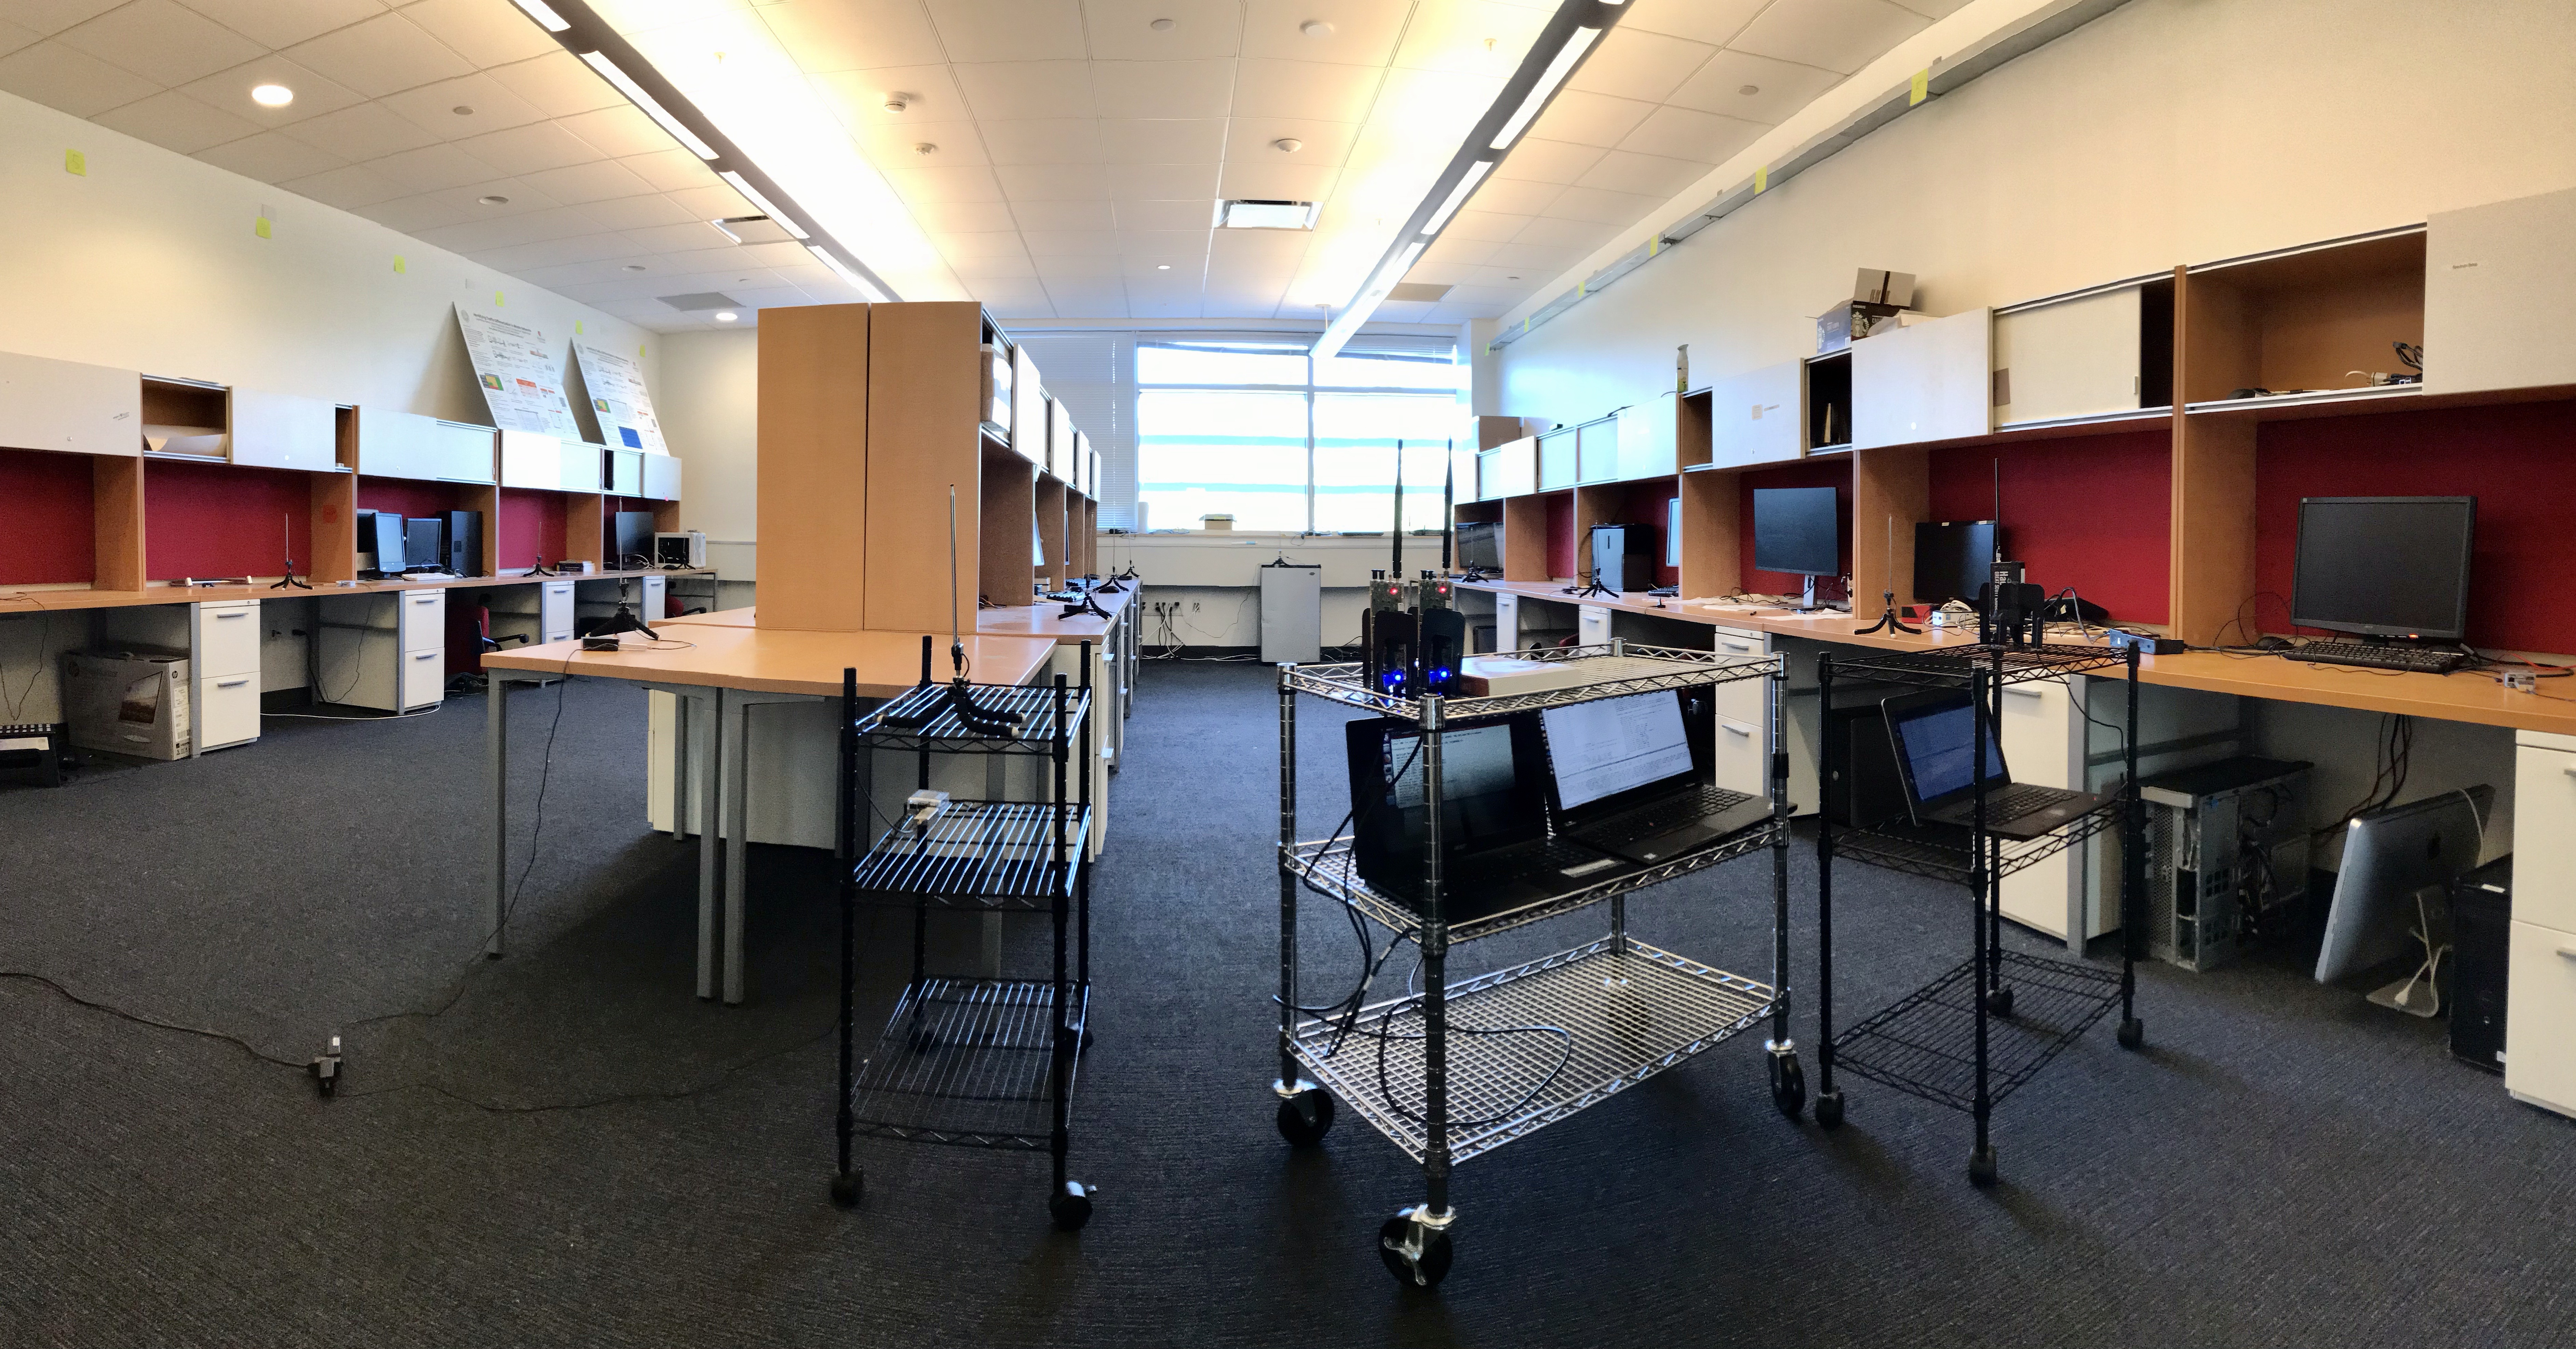
\includegraphics[width=\textwidth]{chapters/ipsn/figures/indoor.jpg}
		\caption{Indoor lab environment}
	\end{subfigure}
	\qquad
	\hspace{-0.15in}
	\begin{subfigure}[t]{0,42\textwidth}
		\includegraphics[width=\textwidth]{chapters/ipsn/figures/floor-plan.png}
		\caption{Floor plan}
	\end{subfigure}
	\caption{Indoor testbed. (a) Our lab used for the indoor testbed, (b) The lab's floor plan.}
	\label{fig:indoor}
\end{figure}

\begin{figure}
	\centering
	\begin{subfigure}[t]{0.585\textwidth}
		\includegraphics[width=\textwidth]{chapters/ipsn/figures/outdoor.jpg}
		\caption{Outdoor parking lot environment]}
	\end{subfigure}
	% \subfloat[Outdoor parking lot environment]{\includegraphics[width=0.585\textwidth]{chapters/ipsn/figures/outdoor.jpg}}
	\qquad
	\hspace{-0.15in}
	\begin{subfigure}[t]{0.33\textwidth}
		\includegraphics[width=\textwidth]{chapters/ipsn/figures/outdoor-sate.png}
		\caption{Satellite}
	\end{subfigure}
	% \subfloat[Satellite]{\includegraphics[width=0.33\textwidth]{chapters/ipsn/figures/outdoor-sate.png}}
	\caption{Outdoor testbed. (a) Parking lot picture, (b)
          Satellite image of the parking lot; the red box is the area
          of the experiment, and the stars are the locations of
          sensing devices during evaluation.}
	\label{fig:outdoor}
\end{figure}

\para{Testbeds.} The {\bf indoor} testbed is built in a lab of our
Computer Science building.  Figure \ref{fig:indoor} depicts the lab
with its floor plan. The red box in the floor plan is the area where
experiments are conducted. The area is 9.6 $\times$ 7.2 $m^2$ (or 2177
square feet) large, with four rows of desks. The middle two rows
are separated by a wooden board. The area is imagined to be divided
into 48 grid cells each of size 1.2m $\times$ 1.2$m$, with the help of
ceiling tiles each of which is 0.6m $\times$ 0.6 $m$. 
%%%%
The {\bf outdoor} testbed is over an open space parking lot.  See
Figure~\ref{fig:outdoor}. The area is 32m $\times$ 32m. We divide the
area into 100 grid cells with each cell representing an area of 3.2m
$\times$ 3.2m. The GPS device returns location in (latitude,
longitude) and the program converts it into coordinates. We use an
outdoor WiFi router and long power cords for network and electrical
connection respectively.
%%%%%%%
During the evaluation, the 18 sensing devices are placed on the ground
and are randomly spread out.


\para{Training.} In both the testbeds, for training (i.e.,
constructing non-interpolated PDs), we first pick 18 random grid cells
and place sensors in their approximate centers. Then, we manually move
the transmitter around in a cart through each of the grid cells. For
the USRP transmitter, we use a gain value of 45 in the indoor
environment and 58 in the outdoor testbed. We use a higher gain for
outdoors to allow the transmitter to have a larger transmission range
in a larger area.
%%%%%%
With each grid cell, the transmitter transmits from 3 to 4 different
points within each grid cell, and for each such location of the
transmitter, the sensors (at the 18 picked locations) gather tens of
signal strength readings. From these readings, we construct a Gaussian
probability distribution from each grid cell location of the
transmitter.
%%%%
More specifically, for a particular grid cell location of the
transmitter, we average over the readings from multiple TX positions
within that particular grid cell---this process of averaging different
positions of the TX inside a grid cell makes the Gaussian
distributions more robust to multipath fading and shadowing. The
overall training process takes an hour for indoors, and about two and
a half hours for outdoors.

\para{Evaluation.}  For evaluation, in both testbeds, we place the 18
sensors at centers of grid cells that are randomly chosen and are
different from the cells chosen for training above. The chosen
locations for the outdoor tested are shown in
Fig.~\ref{fig:outdoor}(b). We choose the intruder's gain/power to be
in the range of [$\pstar-1, \pstar+1$], where $\pstar$ is the
gain/power used during the training phase as mentioned above.
%%%%%
Roughly half of our experiments involve close-by (in the same or
adjacent grid cells) intruders. Localization is done on a laptop which
listens to HTTP requests containing the sensors' observations. 

\subsection{Results}

\begin{figure}
	\centering
	\includegraphics[width=0.7\textwidth]{chapters/ipsn/figures/indoor-error-missfalse.png}
	\caption{Localization performance of varies algorithms in an indoor testbed}
	\label{fig:indoor-error-miss-false}
\end{figure}

\begin{figure}
	\centering
	\includegraphics[width=0.7\textwidth]{chapters/ipsn/figures/outdoor-error-missfalse.png}
	\caption{Localization performance of varies algorithms in an outdoor testbed}
	\label{fig:outdoor-error-miss-false}
\end{figure}

\para{Localization Metrics.}
Figure~\ref{fig:indoor-error-miss-false}-\ref{fig:outdoor-error-miss-false}
show the localization results for the indoor and outdoor testbeds
respectively. Overall, the results indicate that \ouralgo performs the
best across all metrics, with the overall performance gap between
\ouralgo and \splot increasing with the increase in number of
intruders. When the number of intruders is 3, the performance of
\splot is significantly worse than \ouralgo due to a
significantly higher (84\% for indoors and 53\% for outdoors) sum of miss and false-alarm rates and 43\% higher localization error.
%%%%
The \cl algorithm generally performs the worst, but its
performance doesn't have a strong correlation with the increase in the
number of intruders; recall that \cl is given the range of number of
intruders as an extra piece of information compared to the other
algorithms.  In terms of absolute performance, we see that the
localization error of \ouralgo is roughly around 1 or less grid cell,
and the sum of miss-rate and false-alarm is between 5-15\%.

\begin{table}[h]
	\centering
	\caption{Interpolation Mean Absolute Error (MAE) and  Mean Error (ME) in dB for \idw and \ildw}
	\begin{tabular}{c | c c c c}
		\hline\hline
		& \idw & \ildw &  \idw & \ildw \\ 
		Environment & (MAE) & (MAE)  & (ME) &  (ME) \\
		\hline 
		Indoor &  2.6 & 1.7  &  1.7 & 0.25  \\
		Outdoor & 6.2 & 2.7 & 5.8 & 0.48  \\
		\hline %inserts single line
	\end{tabular}
	\label{tab:inter-error}	
\end{table}

\para{Interpolation Error.}
Table \ref{tab:inter-error} show the
interpolation mean absolute error (MEA) as well as mean error (ME) of
\idw and \ildw when the transmitter and receiver are close by (i.e.,
within a distance of 3 grid cells). When the transmitter and receiver
are far away, the difference of \idw and \ildw is small and thus not
shown.  We see that when compared with \idw, our \ildw interpolation
scheme decreased the mean absolute error by 35 percent in the indoor
environment and 56 percent in the outdoor environment.  In terms of
mean error, \ildw reduced the error compared to \idw by as large as 86
percent and 92 percent respectively. This is because \idw
mostly tends to estimate the value to be larger than the ground truth,
while \ildw's estimates are more even across the ground truth.

\begin{table}[ht]
	\caption{Power Prediction Mean Absolute Error (MAE) and Mean Error (ME) in dB for indoor and outdoor testbed}
	\centering
	\begin{tabular}{c | c c c c}
		\hline\hline
		& Indoor & Outdoor & Indoor  & Outdoor  \\
		\# Intruder  & (MAE)   &    (MAE)   &  (ME)  &   (ME)     \\
		\hline
		1 & 0.34 & 0.50 & -0.02 &  0.02 \\ 
		2 & 0.57 & 0.63  &  0.10 & 0.54\\
		3 & 0.77 & 0.90 & 0.49 & 0.76\\
		\hline %inserts single line
	\end{tabular}
	\label{table:power-error}
\end{table}

\para{Intruder Power.}  Table ~\ref{table:power-error} show the errors in the predicted powers of
the intruders in \ouralgo. We see that the outdoors have a slightly
higher power prediction error, likely because of a larger number of
grid cells. We also note that with the increase in the number of
intruders, the error in predicted power increases.





